\documentclass[conference]{IEEEtran}
\IEEEoverridecommandlockouts
% The preceding line is only needed to identify funding in the first footnote. If that is unneeded, please comment it out.
\usepackage{cite}
\usepackage{url}
\usepackage{graphicx, float}
\usepackage{amsmath,amssymb,amsfonts}
\usepackage{algorithmic}
\usepackage{graphicx}
\usepackage{textcomp}
\usepackage{xcolor}

\graphicspath{{Figures/}}
\def\BibTeX{{\rm B\kern-.05em{\sc i\kern-.025em b}\kern-.08em
    T\kern-.1667em\lower.7ex\hbox{E}\kern-.125emX}}
\begin{document}

\title{Research Paper: Cyberattack Case Study \\CIS 3360-Security in Computing\\Fall 2025\\
{\footnotesize Instructor: Jie Lin, Ph.D.}
\thanks{}
}

\author{{ Derek Oliveira}\\
\IEEEauthorblockA{\textit{department of engineering and computer science} \\
Orlando, United States of America \\
de937084@ucf.edu}
}

\maketitle

\begin{abstract}
The SolarWinds cyber breach, disclosed in December 2020, stands as one of the most significant cyber-espionage
incidents of the modern era. Through a sophisticated supply-chain compromise of SolarWinds' Orion platform, 
the state sponsored hacker group NOBELIUM gained persistent and covert access to U.S. government agencies,
corporations, and critical service providers. This paper examines the historical context, motives, and technical execution
of the attack that gave persistent anonymous access to SolarWinds' build environment, dubbed SUNBURST, demonstrating how the breach not 
only infiltrated high level networks but also undermined global trust in software ecosystems. By analyzing
NOBELIUM's tactics and the far-reaching consequences of the intrusion, I argue that the SolarWinds incident
represents a makeup call moment in cybersecurity. It highlights the vulnerability of supply chains, exposes
the limitations of traditional defense mechanisms, and guided us to new industry standards that shape the cybersecurity
landscape today. 
\end{abstract}

\begin{IEEEkeywords}
SUNBURST, formatting, style, styling, insert
\end{IEEEkeywords}

\section{Introduction}

% Identify the attack, when/whom it affected, why it meets the significance 
% criteria, your thesis, and a brief roadmap.

On December 13, 2020, SolarWinds, A Texas based technology company that develops network monitoring and IT 
infrastructure management software, announced what would become the most consequential cyber intrusion in history.
The breach focused on exploiting their Orion software, SolarWinds' main network monitoring platform used by U.S. 
government agencies, defense contractors, Fortune 500 corporations, and critical national service providers. 
The attackers, latter dubbed NOBELIUM by Microsoft's Threat Intelligence center (MSTIC) discovered to be
state sponsored attacker group backed by Russia, pursued espionage rather than economic gains.
SolarWinds itself was not the ultimate target, thou. Instead, its compromised software supply chain became the conveyor belt for malicious 
code that infiltrated networks of its customer base undetected for over a year. There were many exploits deployed in this attack, but for the 
scope of this research I will focus on the "SUNBURST" exploit.

By the time the intrusion was detected, NOBELIUM had already guaranteed their persistent, undetected access to email servers,
sensitive repositories, and classified communications for about one year. What followed was not a simple data breach, but a calculated and methodical 
campaign of cyber-espionage that exploited trust and used it as a mask for malicious intent. The SolarWinds incident was deemed a 
significant cyberattack not only because of its scale and sophistication, but also because of the national security risk it posed and 
the trust it shattered in the global technology leaders that are the watchdogs of our virtually connected world.

I argue that the SolarWinds breach represents a turning point in cybersecurity. It revealed the vulnerabilities of software supply 
chains, exposed the weakness of existing detection systems, and forced governments and corporations to rethink the resilience of their 
networks and how they can restructure themselves for reduced impact. To explore this claim, I will first outline the historical 
background and motives of NOBELIUM, then examine the technical methods of the SUNBURST intrusion, followed by an analysis of the attack's distinct 
features, its broader geopolitical implications and if the attack's patterns are still in use today. Finally, I will evaluate the lessons 
learned and how this incident reshaped modern approaches to cyber defense.


\section{Background}
%History of Development (actor/group, prior incidents, sponsorship, timeline) 
%and Purpose & Motivation (financial, political, espionage, disruption).
\subsection{NOBELIUM}
NOBELIUM, or as they were previously known; APT29/UNC2452/Cozy Bear/Midnight Blizzard/The Dukes,
are a Russian based threat actor attributed by the U.S. and European leaders as the foreign
intelligence service of the Russian Federation\cite{Microdoft2024NOBELIUM}. NOBELIUM can be traced back
to 2013, when European and American ministries of foreign affairs reported data breaches and theft of data 
through an incident that was latter named "Operation Ghost."\cite{MITREFirstNOBELIUMAttack} NOBELIUM is known for manipulating trust
withing security systems, falsifying digital certificates, virtually impersonating IT managers, and distorting security protocols
to reach their goals. These operations and tactics demonstrated NOBELIUM's strategic focus on infiltrating
high value targets and security long-term access to sensitive information.\\
\subsection{History of Development}
The SolarWinds campaign unfolded over an extended timeline. Initial reconnaissance and infiltration of SolarWinds'
infrastructure likely began as early as September 2019\cite{MicrosoftDeepDiveSOLORIGATE}, with the attackers
quietly embedding themselves into the company's software build process. By March 2020, malicious updates of the Orion
software, later dubbed SUNBURST or SOLORIGATE, were digitally signed and distributed to SolarWinds' global customer base.
For months, the attackers maintained undetected access, refining their foothold and carefully selecting targets before the 
public disclosure on December 12, 2020. This deliberate pacing highlights NOBELIUM's patient and methodical approach to 
cyber-espioage.
\begin{figure}[H]
    \centering
    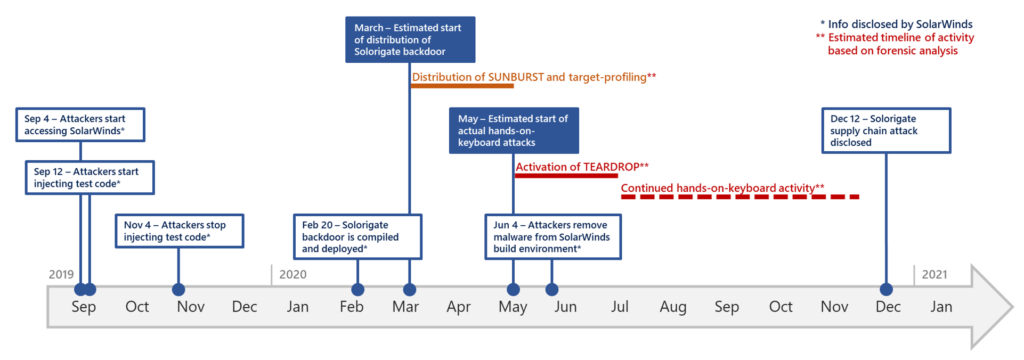
\includegraphics[width=3in]{Timeline-of-Solorigate-attacks.png}
    \caption{Image created by the MSTIC team on the timeline of events that led to the discovery of the SolarWinds
    breach.\\Source: \cite{MicrosoftDeepDiveSOLORIGATE} }
    \label{fig:Timeline-of-Solorigate-attacks}
\end{figure}





\section{Analysis}
%Intended Usage Domain & Penetration Strategy 
%(industry/target environment, initial access, TTPs) 
%and Distinctive Features (innovations, what made it effective/different).


Analysis text here.


\section*{Discussion}
% Active Descendants (whether methods persist/evolved), 
% full CIA triad impact, broader consequences, preventive and 
% punitive responses, lessons learned.


Discussion text here.

\section{Conclusion}
%key findings, recommendations, future implications, and limitations.


Conclusion text here.

\section*{Citations}

Please number citations consecutively within brackets \cite{b1}. The 
sentence punctuation follows the bracket \cite{b2}. Refer simply to the reference 
number, as in \cite{b3}---do not use ``Ref. \cite{b3}'' or ``reference \cite{b3}'' except at 
the beginning of a sentence: ``Reference \cite{b3} was the first $\ldots$''

Number footnotes separately in superscripts. Place the actual footnote at 
the bottom of the column in which it was cited. Do not put footnotes in the 
abstract or reference list. Use letters for table footnotes.

Unless there are six authors or more give all authors' names; do not use 
``et al.''. Papers that have not been published, even if they have been 
submitted for publication, should be cited as ``unpublished'' \cite{b4}. Papers 
that have been accepted for publication should be cited as ``in press'' \cite{b5}. 
Capitalize only the first word in a paper title, except for proper nouns and 
element symbols.

For papers published in translation journals, please give the English 
citation first, followed by the original foreign-language citation \cite{b6}.

\begin{thebibliography}{00}
\bibitem{Microdoft2024NOBELIUM} Microsoft, ``Nation State Actors Midnight Blizzard,'' \emph{Microsoft Security Insider}, Jan. 25, 2024. [Online]. Available: \url{https://www.microsoft.com/en-us/security/security-insider/threat-landscape/midnight-blizzard}. [Accessed: Sept. 29, 2025].
\bibitem{MITREFirstNOBELIUMAttack} MITRE, ``Operation Ghost (Campaign C0023),'' \emph{MITRE ATT\&CK}. [Online]. Available: \url{https://attack.mitre.org/campaigns/C0023/}. [Accessed: Sept. 29, 2025].
\bibitem{MicrosoftDeepDiveSOLORIGATE} Microsoft Cyber Defense Operations Center and Microsoft Threat Intelligence, ``Deep Dive into the Solorigate Second-Stage Activation: From SUNBURST to TEARDROP and Raindrop,'' \emph{Microsoft Security Blog}, Jan. 20, 2021. [Online]. Available: \url{https://www.microsoft.com/en-us/security/blog/2021/01/20/deep-dive-into-the-solorigate-second-stage-activation-from-sunburst-to-teardrop-and-raindrop/}. [Accessed: Sept. 29, 2025].
\bibitem{b4} K. Elissa, ``Title of paper if known,'' unpublished.
\bibitem{b5} R. Nicole, ``Title of paper with only first word capitalized,'' J. Name Stand. Abbrev., in press.
\bibitem{b6} Y. Yorozu, M. Hirano, K. Oka, and Y. Tagawa, ``Electron spectroscopy studies on magneto-optical media and plastic substrate interface,'' IEEE Transl. J. Magn. Japan, vol. 2, pp. 740--741, August 1987 [Digests 9th Annual Conf. Magnetics Japan, p. 301, 1982].
\bibitem{b7} M. Young, The Technical Writer's Handbook. Mill Valley, CA: University Science, 1989.
\end{thebibliography}
\vspace{12pt}
\color{red}
IEEE conference templates contain guidance text for composing and formatting conference papers. Please ensure that all template text is removed from your conference paper prior to submission to the conference. Failure to remove the template text from your paper may result in your paper not being published.

\end{document}
About
About us
Careers
Blog
Solutions
For business
For universities
For government
For publishers
Customer stories
Learn